\documentclass[a4paper,twocolumn,10pt]{article}
\usepackage[utf8x]{inputenc}
\usepackage[spanish,es-tabla]{babel}
\usepackage{amsmath,amsfonts,amssymb}
\usepackage{graphicx}
\usepackage{flushend}
\usepackage{multicol}
\usepackage{multirow}
\usepackage{xcolor,colortbl}
\usepackage{setspace}
\author{Brenda Romero Salcedo}
\title{Proyecto final. Review Científico sobre VIH}
\date{16 de Octubre de 2018}
\begin{document}
\twocolumn[
\begin{@twocolumnfalse}
\vspace*{-3cm}
\maketitle
\vspace*{-1cm}
\begin{center}\rule{0.9\textwidth}{0.1mm}\end{center}
\begin{abstract}
\begin{quote}
\normalsize La infección-enfermedad por VIH/SIDA es una afección crónica transmisible de tipo progresivo y causa viral, en la cual se establece una relación muy diversa entre huésped y virus, que finalmente condiciona la aparición de procesos morbosos oportunistas o tumores raros, o ambos\cite{Castillo2004}.
El VIH/SIDA es una pandemia. A nivel mundial para el año 2002 se estimaba 3.1 millones de muertes por VIH/SIDA, 42 millones de adultos y niños viviendo con el VIH/SIDA y 5 millones de casos nuevos de infección por el VIH en estos grupos, de los cuales 150,000 corresponderían a América Latina\cite{LinaMariaVera2004}.En España hay aproximadamente 130.000 infectados por el VIH, lo que representa una prevalencia de infección de 2,7-3,7 casos por 1.000 habitantes, y se han notificado casi 80.000 casos de SIDA hasta el 30 de septiembre de 2010. En los nuevos diagnósticos de infección por el VIH, la transmisión en hombres que mantienen relaciones sexuales con hombres es la más frecuente, seguida de la heterosexual, y finamente la producida en usuarios de drogas inyectadas (UDI) \cite{Marco2012}.\\
La neuropatía periférica es la complicación neurológica más frecuente en la infección por VIH \cite{Ferri2002}.  Las diferentes situaciones clínicas asociadas al VIH/sida, que se dan en el transcurso de la infección, aumentan considerablemente el riesgo de malnutrición y repercuten en el consumo, la digestión y el aprovechamiento de los alimentos \cite{Herrera2004}. \\ \\
{\bfseries Palabras clave:} VIH, Infectados, Pandemia, Transmisión, Neuropatía, Malnutrición.
\end{quote}
\begin{center}\rule{0.9\textwidth}{0.1mm}\end{center}
\vspace*{0.5cm}
\end{abstract}
\end{@twocolumnfalse}
]
\section{Introducción}
El VIH/SIDA es una pandemia. Las estadísticas actuales muestran que los jóvenes entre 15 y 24 años son los más vulnerables. En Colombia, 7,497 jóvenes entre 10 y 30 años de edad viven con VIH/SIDA \cite{LinaMariaVera2004}. En España hay aproximadamente 130.000 infectados por el VIH, lo que representa una prevalencia de infección de 2,7-3,7 casos por 1.000 habitantes, y se han notificado casi 80.000 casos de SIDA hasta el 30 de septiembre de 2010. En el año 2009 se diagnosticaron 2.264 nuevos casos de infección, que suponen una tasa de 79,3/millón de habitantes, similar a la de países de nuestro entorno, como Francia, Bélgica o Irlanda, e inferior a las de Estonia, Letonia, Portugal y el Reino Unido, pero superior a la media del conjunto de países de la Unión Europea \cite{Marco2012}.A nivel mundial para el año 2002 se estimaba 3.1 millones de muertes por VIH/SIDA, 42 millones de adultos y niños viviendo con el VIH/SIDA y 5 millones de casos nuevos de infección por el VIH en estos grupos, de los cuales 150,000 corresponderían a América Latina \cite{LinaMariaVera2004}. \\ \\
La infección-enfermedad por VIH/SIDA es una afección crónica transmisible de tipo progresivo y causa viral, en la cual se establece una relación muy diversa entre huésped y virus, que finalmente condiciona la aparición de procesos morbosos oportunistas o tumores raros, o ambos\cite{Castillo2004}. En los nuevos diagnósticos de infección por el VIH, la transmisión en hombres que mantienen relaciones sexuales con hombres es la más frecuente, seguida de la heterosexual, y finalmente la producida en usuarios de drogas inyectadas(UDI). Aunque en España, en los primeros años de la epidemia la infección por el VIH afectó mayoritariamente a los UDI, la disminución de nuevos casos en este colectivo viene ocurriendo desde la década de los noventa, probablemente por el menor uso de la vía endovenosa en los heroinómanos, por la extensión de los programas de tratamiento con metadona, por las campañas educativas, y por la menor incorporación de jóvenes al consumo de drogas inyectadas. La reducción de la transmisión del VIH en los UDI también se ha observado en el colectivo de los presos, que ha presentado importantes cambios sociológicos en los últimos años: modificación del patrón de consumo en drogodependientes españoles, con menor uso de la vía parenteral, y aumento de reclusos inmigrantes, que son generalmente menos UDI. Es muy posible que estos cambios sociológicos hayan supuesto importantes modificaciones en la prevalencia de infección por el VIH en población penitenciaria \cite{Marco2012}.
\begin{figure}[htb]
\centering
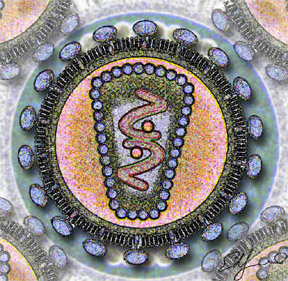
\includegraphics[width=0.3\textwidth]{./VIH1}
\caption {VIH \cite{Wikipedia2018}}
\label{fig:VIH}
\end{figure}
\\ 
El síndrome de la inmunodeficiencia adquirida (SIDA) es la última etapa clínica de la infección por el virus de la inmunodeficiencia humana (VIH), que se puede transmitir por vía sexual, por transfusión sanguínea y de la madre al hijo, ya sea durante el embarazo, el parto o la lactancia materna. A partir del momento en que el virus entra al cuerpo humano pueden pasar de dos semanas a tres meses antes de que apa- rezcan anticuerpos en su sangre. En promedio, la enfermedad tiene un período de incubación de diez años, lo que implica que una persona puede transmitir el virus sin saber que está infectada \cite{LinaMariaVera2004}. \\ \\
La neuropatía periférica es la complicación neurológica más frecuente en la infección por VIH. Existe una correlación significativa entre otras complicaciones neurológicas de la infección por VIH y la presencia neuropatía periférica. Los estudios establecen una incidencia que varía entre el 35 y 17 de cada cien. Las diferentes situaciones clínicas asociadas al VIH/sida, que se dan en el transcurso de la infección, aumentan considerablemente el riesgo de malnutrición y repercuten en el consumo, la digestión y el aprovechamiento de los alimentos. Las infecciones en la boca y en el tracto digestivo, las náuseas o el vómito, la diarrea y la pérdida de peso son más tolerados con un buen estado nutricional \cite{Herrera2004}.
\paragraph{Prevalencia}
\begin{figure*}[htb]
\centering
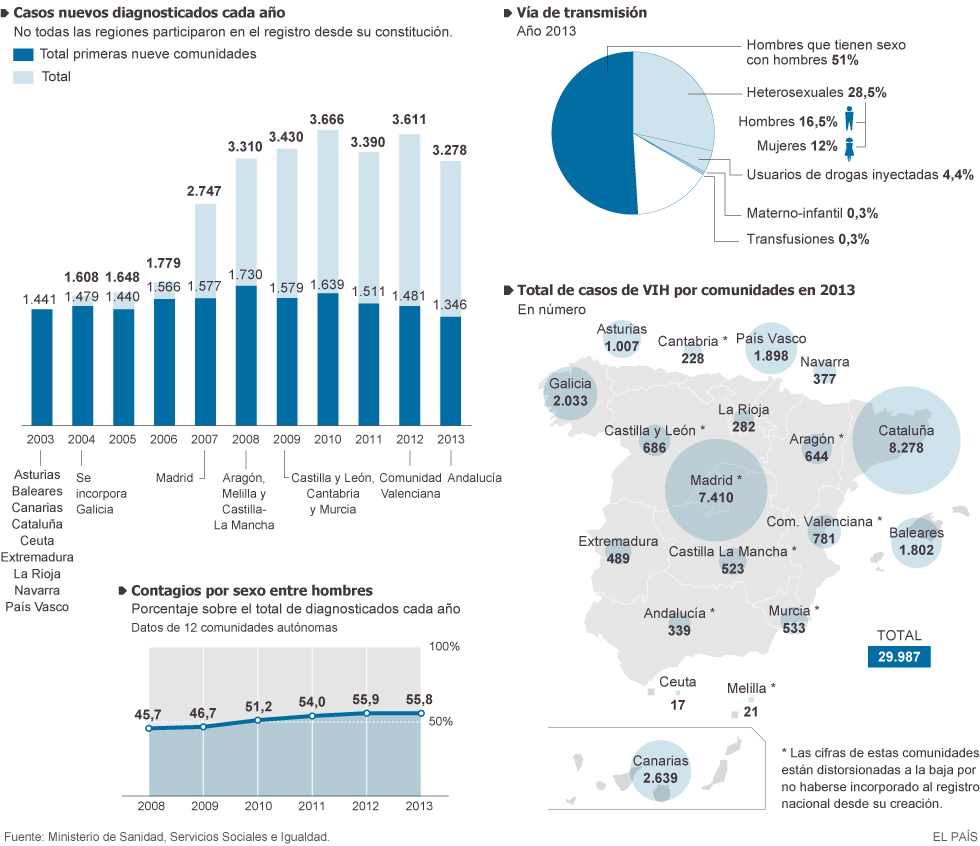
\includegraphics[width=0.9\textwidth]{./sida}
\caption{Mapa del VIH en España. \cite{Benito2014}}
\label{fig:VIH}
\end{figure*}
\paragraph{prevalencia}
\begin{table}[htbp]
\begin{center}
\begin{tabular}{|c|c|}
\hline 
{\cellcolor[gray]{0.7} \bfseries Personas} & {\cellcolor[gray]{0.7} \bfseries Frecuencia} \\ \hline 
Hombre Sexo Hombre & 53,1 \\ \hline
Heterosexual & 26,1 \\ \hline
Inyección de drogras & 3,6 \\ \hline
Transmisión vertical & 0,18 \\ \hline
Nacidos fuera de España & 33,6 \\ \hline
Mediana de edad & 36 \\ \hline
Hombre & 83,9 \\ \hline
Mujer & 16,1 \\ \hline 
Total de diagnosticados & 3353 \\ \hline 
\end{tabular}
\caption{Prevalencia en España \cite{Molina2018}}
\label{tabla:Prevalencia}
\end{center}
\end{table}
\paragraph{Neuropatía} 
A pesar de la alta tasa de incidencia y prevalencia, su diagnóstico y tratamiento a menudo son obviados. Son entidades que no ponen, generalmente, en peligro la vida, pero son generadoras de alta morbilidad \cite{Ferri2002}. \\ \\
Existen al menos 6 patrones de manifestación de neuropatía periférica asociada a VIH: Polineuropatía simétrica distal, Polirradiculopatía progresiva, Mononeuropatía múltiple, Neuropatía autonómica, Síndrome de linfocitosis difusa infiltrante \cite{Ferri2002}.
\paragraph{Malnutrición}
Es vital desde el diagnóstico de la enfermedad asegurar una alimentación correcta y no esperar a que surja un problema que dé la alarma, como, por
ejemplo, una pérdida de peso. Una nutrición adecuada es una condición necesaria para mantener un buen nivel de salud.Una buena nutrición tiene los siguientes objetivos\cite{Herrera2004}:
\begin{itemize}
\item{\mdseries \itshape Conservar o mejorar el estado nutricional}
\item{\mdseries \itshape Mejorar la calidad de vida}
\item{\mdseries \itshape Facilitar la recuperación de infecciones}
\item{\mdseries \itshape Mejorar la tolerancia a la medicación}
\end{itemize}
\begin{table*}[htb]
\begin{center}
\begin{tabular}{|p{0.5\textwidth}|p{0.5\textwidth}|}
\hline \hline
{\cellcolor[gray]{0.7} \bfseries Alimentos recomendados} & {\cellcolor[gray]{0.7} \bfseries  Alimentos prohíbidos} \\ \hline \hline
Tostadas, espaguetis, macarrones, pasta de sopa, arroz, patatas & Cereales integrales, garbanzos,lentejas, alubias \\ \hline
Verduras cocidas en pequeña cantidad y mezcladas con otros alimentos & Verduras como plato y ensaladas \\ \hline
Leche y derivados. Flan & Quesos secos\\ \hline
Pollo, ternera, pescados, jamón dulce,embutido de pavo, tortilla francesa & Otras carnes y mariscos\\ \hline
Raciones pequeñas de frutas & Naranja, melocotón, melón,
sandía, limón \\ \hline
Azúcar, mermelada, bollería, galletas & Pastelería, chocolate \\ \hline
Condimentos de hierbas, cebolla,
laurel & Pimienta, curry \\ \hline
Infusiones de manzanilla, anís,
café suave, té & Cerveza, bebidas alcohólicas
y carbonatadas, café cargado\\ \hline
\end{tabular}
\caption{Alimentos recomendados para evitar la malnutrición. \cite{Herrera2004}}
\label{tabla:Alimentos}
\end{center}
\end{table*}
\section{Métodos}
Se hizo una revisión de una serie de artículos y libros relacionados con diversas investigaciones sobre la prevalencia \cite{Marco2012}, transmisión \cite{LinaMariaVera2004}, \cite{Sepulveda-Amor1995}, infección-transmisión \cite{Castillo2004}, trastornos como la neuropatía dolorosa \cite{Ferri2002} y la malnutrición \cite{Herrera2004}. 
\section{Discusión}
Con respecto a la Neuropatía dolorosa, el problema en el uso de medicación junto con el tratamiento retroviral es importante, en cuanto, que la disminución de la eficacia de los retrovirales por interacción farmacológica ocasiona una progresión virológica de la enfermedad. El fármaco ideal es aquel que se una poco a proteínas, y por tanto no tenga una interacción en el locus de unión, ni se afecte por la hipoalbuminemia; y además que no produzca inducción de los citocromos P450, que en el caso de los inhibidores de las proteasas es donde ocurre su metabolismo. Es por ello que l tratamiento del dolor neuropático está en continuo proceso de cambio y renovación. Además se añade la gran variabilidad en la respuesta individual a los distintos grupos farmacológicos, e incluso a las distintas drogas del mismo grupo. El tratamiento enfocado al control de los síntomas en monoterapia con un agente bien escogido o en politerapia con una combinación de fármacos que actúen mediante distintos mecanismos, sería el tratamiento ideal.\\ \\
Un hecho importante a tener en cuenta es la polimedicación de la que son objetos estos pacientes: retrovirales, en esquemas de terapia combinada; tratamientos profilácticos; tratamientos de la enfermedad o del contacto con la tuberculosis, etc \cite{Ferri2002}. \\ \\
Finalmente, es evidente la relación entre la alimentación, la nutrición y el proceso de la enfermedad crónica. Tal es el caso de los pacientes con la infección por VIH (virus de inmunodeficiencia humana). La comunidad científica reconoce que los conocimientos y el cuidado nutricional pueden contri-
buir a mantener la salud y a paliar los efectos de una enfermedad crónica. Existe una demanda por parte tanto de los pacientes como de los profesio-
nales implicados en su cuidado de que se les proporcione una información útil y científicamente validada. Hay que tener en cuenta que la alimentación, aunque sea la más cotidiana, desempeña un papel importante, aportando a los pacientes seropositivos paliativos específicos, en una situación que afecta a su salud, a su nutrición y a los efectos secundarios de su tratamiento \cite{Herrera2004}.
\paragraph{Módelo Matemático} 
El modelo está caracterizado por tres ecuaciones \cite{Kirschner1996}, las cuales se desarrollan a continuación: \\
\begin{center}
\doublespacing
{\itshape \underline{1ª Ecuación:}} \\
$dT(t)/dt = s(t)-\mu_TT(t)+ \\ 
r(T(t)V(t))/(C+V(t))- K_VT(t)V(t),$ \\ 
{\itshape \underline {2ª Ecuación:}} \\
$dT^i(t)/dt = K_vT(t)V(t)-\mu_T^iT^i(t)-\\
r((T^i)(t)V(t))/(C+V(t)),$ \\
{\itshape \underline {3ª Ecuación:}} \\
$dV(t)/dt=Nr(T^i(t)V(t))/C+V(t)-k_TT(t)V(t)+ \\
(gvV(t)/b+V(t)). $ \\
\end{center}
\section{Conclusión}
En relación a la Neuropatía dolorea el fármaco ideal sería aquel que pudiese ser administrado en monoterapia, que tuviese pocas o ninguna in-
teracción farmacológica con el resto de medicaciones que toma el paciente, con buena tolerancia y con perfiles de seguridad y eficacia altos. \\ \\
En lo que respecta al tándem alimentación-nutrición efectuado de una forma correcta contribuye a mantener y/o mejorar la situación nutricional del paciente, a prevenir su deterioro y a paliar los síntomas que pueden aparecer en el desarrollo de su enfermedad, obteniendo así una mejora considerable de su calidad de vida \cite{Herrera2004}.
\bibliographystyle{plain}
\bibliography{bibliografia}
\end{document}
